\documentclass{article}
\usepackage{graphicx, listings, noweb, textcomp, amsmath, xcolor, graphicx}
\lstset{
    frame=single,
    breaklines=true,
    postbreak=\raisebox{0ex}[0ex][0ex]{\ensuremath{\color{red}\hookrightarrow\space}}
}
\graphicspath{ {images/} }

\begin{document}

\title{Literate Programming Report}
\author{Kevin Carmona-Murphy, 1059136}

\maketitle

\begin{abstract}
\textbf{roadnet} is a Ruby based compiler for converting an XML description of a road network into an HTML/SVG visual representation. This document outlines the methodology, languages and frameworks used, as well as implenetation and testing steps.
\end{abstract}

\section{Summary}
\textbf{roadnet} is the name given to a tool which allows for the generation of simple graphical road networks using a specially developed road topology language. This tool converts an XML file containing the hierarchy of the road network into an HTML page displaying the network from a bird's-eye viewpoint, using SVG drawings. Three different road types are supported, including a two-lane road, a local street, and a four lane avenue. Road length, intersection radius, and intersecting angle offsets are the parameters that are specifiable, in addition to the structure of the network, via the XML file.

\subsection{Problem Inspiration}
The inspiration for the tool stems from a pass-time I once cherished as a child. I would often spend hours sketching small neighbourhoods onto a large piece of drafting paper. Attention to detail was especially evident in how I drew the roads; from a bird's eye perspective, lane widths were meticulously calculated and enforced with a ruler through the entirety of my drawings.\\

Attempting to bring rekindle that hobby and bring it into the digital world is the motivation for such a tool. While of no practical purpose for transportation engineers, it offers an academic and practical insight into the fundamentals of compiler design with recursion, using a modern high-level language.

\section{Languges \& Tools}
The compiler transforms an XML file into an HTML file with embedded SVG graphics. XML was chosen as the source because it allows one the freedom to write nested hierarchies with tags that describe attributes. This is important given that a road topology is a network of elements that are often repeated and are always connected to one another. An XML file assures that each element has a parent, just like each segment of road generally intersects with another.\\

SVG within HTML is used as the output representation because it is a very widely available and performant markup language which is compatible across platforms. Using SVG, \textbf{roadnet} is able to easily create paths that represent lane markings, road edges, and intersections.\\

The program is written in Ruby in order to take advantage of the excellent Nokogiri gem which makes the task of parsing elements in XML and HTML files a breeze. In the implementation, Nokogiri parses the XML file recursively, drawing the appropriate paths in SVG as it descends the parse tree.

\section{Resources}
Various resources were consulted over the course of the development of the tool. \\

Resources consulted over the course of the project:
\begin{itemize}  
\item \textbf{General inspiration:} http://programmers.stackexchange.com/questions/165543/how-to-write-a-very-basic-compiler
\item \textbf{Nokogiri docs:} https://github.com/sparklemotion/nokogiri
\item \textbf{Nokogiri cheatsheet:} https://github.com/sparklemotion/nokogiri/wiki/Cheat-sheet
\item \textbf{SVG primer:} http://www.w3schools.com/svg/svg\_examples.asp
\item \textbf{LaTeX information:} https://en.wikibooks.org/wiki/LaTeX
\item \textbf{NoWeb literature:} http://www.literateprogramming.com/noweb\_hacker.pdf
\end{itemize}

\section{Implementation}

\subsection{Getting Started}

Running \textbf{roadnet} is very simple. In the directory where parser.rb is found, simply execute the following command:\\

\begin{lstlisting}[language=bash]
  $ ruby parser.rb -f rd.xml
\end{lstlisting}.\\

The -f command line option is necessary - it specifies the road topology xml file. An -o flag is optional, it specifies the output file. The default output file is diagram.html

\subsection{The XML Source}

The XML file must have exactly one \textlangle network\textrangle\ root tag, followed by any number of nested structures comprising of \textlangle road\textrangle, \textlangle avenue\textrangle, or \textlangle street\textrangle\ tags. Including other tags will raise an error. A parent tag of child elements suggests that the child elements are connected via an intersection to the end of the parent tag.\\

There are four specifiable attributes. The \em{intersection-offset}\em\ and \em{intersection-radius}\em\ are intersection level attributes, and specify properties pertaining to an intersection, while the \em{length}\em\ attribute and \em{angle-offset}\em\ specify properties of a network link (be it a road, street, or avenue). \em{intersection-offset}\em\ is specified in degrees, and rotates the intersection and all jutting links by x degrees. \em{intersection-radius}\em\, specified in pixels, dicates the radius an intersection. \em{angle-offset}\em\ rotates the specific link on which it is called x degrees clockwise. \em{length}\em\ is self explanatory, its dimensions are in pixels.\\

Here is an example XML file illustrating the abovementioned properties:\\

\begin{lstlisting}[language=xml]
<?xml version="1.0" encoding="UTF-8"?>

<network intersection-radius="100">
	<avenue>
	</avenue>
	<road intersection-offset="180" angle-offset="-20" intersection-radius="20">
		<road>
		</road>
		<street>
		</street>
	</road>
	<road>
	</road>
	<road>
		<street>
		</street>
		<street length="400" >
			<road>
			</road>
			<road>
			</road>
			</street>
		<street>
		</street>
	</road>
	<street>
	</street>
</network>
\end{lstlisting}.\\

Due to the recursive tree-like structure of the XML file, no cycles are permitted in the road network. That is, a nested link cannot connect with with another beyond its immediate siblings. In other words, the set forms a minimum spanning tree, and is divergent, rather than convergent.

\subsection{Ruby Program}

There are three dependencies that must be installed using a tool such as \textbf{bundler}\textbf\ before running the program. These dependencies include \textbf{nokogiri},  \textbf{optparse}, and \textbf{solid\_assert}.\\

The below code executes the option parser which looks for the command line arguments specifying the input xml file, and an optional output html file. If the input file is missing, or there are abnormal command line arguments, and error is thrown and the program is aborted.\\

\begin{lstlisting}[language=ruby]
#!/usr/bin/env ruby

require 'rubygems'
require 'bundler/setup'

require 'nokogiri'
require 'optparse'
require 'solid_assert'

SolidAssert.enable_assertions

options = {}

optparse = OptionParser.new do |opts|
	opts.banner = "Usage: parser.rb -f <xml filename> [ -o <output filename> ]"
	opts.on('-f', '-x', '--xml input-filename', 'XML file name') { |v| options[:filename] = v }
	opts.on('-o', '-h', '--html output-filename', 'HTML file name') { |v| options[:output] = v }
end

begin
	optparse.parse!
	mandatory = [:filename]
	missing = mandatory.select{ |param| options[param].nil? }
	unless missing.empty?     
		puts "Missing options: #{missing.join(', ')}"  
		puts optparse                                    
		exit               
	end  
rescue OptionParser::InvalidOption, OptionParser::MissingArgument 
	puts $!.to_s # Friendly output when parsing fails
	puts optparse                                                     
	exit      
end
\end{lstlisting}.

The next section of code opens the XML for parsing using Nokogiri, a parsing library for HTML and XML files. It sets strict options on the file, mandating a well-formed XML file that is free of errors. If errors are detected, the program aborts.\\

Several constants are also set in this part of the program. Notice that these variables begin with an ampersand - this is Ruby's way of telling the user that these variables have a global scope.\\

\begin{lstlisting}[language=ruby]
begin
	@xml = Nokogiri::XML(File.open(options[:filename])) do |config|
		config.options = Nokogiri::XML::ParseOptions::STRICT | Nokogiri::XML::ParseOptions::NONET
	end
rescue Nokogiri::XML::SyntaxError => e
	puts "caught exception: #{e}"
end

begin assert @xml.root.name == "network" rescue abort "Ensure that the <network> tag is at the root" end

#Constants
@default_length = 200
@lane_width = 20
@intersection_radius = 50
\end{lstlisting}.

The next section is the most important - it comprises the bulk of the program's logic - the recursive function definition. In \em{draw\_intersection(node, html, cx, cy)}\em, paths are created in an html object passed into the function. \em{node}\em\ is the current "intersection" being drawn, and changes based on the context of execution (parent vs child elements). \em{cx and cy}\em\ are the origin co-ordinates of the interesection.\\

The function begins by setting up some arrays, which are used for keeping track of the total size taken up by the SVG objects. An angle is computed based on the number of children nodes that will spawn off from the intersection. Other specifiable attributes are initialized next. Finally, we reach a loop structure which iterates over the child elements. Different numbers of lines are drawn depending on the road type. At the bottom, the width and height calculations of the bounding frame are made based on the results from the recursive calls to the child elements.\\

\begin{lstlisting}[language=ruby]
def draw_intersection(node, html, cx, cy)
	
	width_arr = Array.new
	height_arr = Array.new
	
	max_width = 0
	max_height = 0
	min_width = 0
	min_height = 0
	
	angle = 2*Math::PI / node.elements.size
	
	angle_offset = node.key?("angle-offset") ? (node.attribute("angle-offset").value.to_f)*Math::PI/180 : 0
	
	intersection_offset = node.key?("intersection-offset") ? (node.attribute("intersection-offset").value.to_f)*Math::PI/180 : 0

	intersection_radius = node.key?("intersection-radius") ? (node.attribute("intersection-radius").value.to_f) : @intersection_radius
	
	html.circle(:cx => cx, :cy => cy, :r => intersection_radius, :stroke => "red", :fill => "white")
	
	node.elements.each_with_index do |node, index|
		
		length = node.key?("length") ? (node.attribute("length").value.to_f) : @default_length
		
		ang = (angle + angle_offset)*index + intersection_offset
		x_dist = Math.cos(ang)*length
		y_dist = Math.sin(ang)*length
		
		x_radius = Math.cos(ang)*intersection_radius
		y_radius = Math.sin(ang)*intersection_radius
		
		x_start = cx + intersection_radius*Math.cos(ang)
		y_start = cy + intersection_radius*Math.sin(ang)
					
		if node.name == "road"
			#draw three lines

			x_start_1 = x_start + @lane_width*Math.cos(ang - Math::PI/2)
			x_start_2 = x_start + @lane_width*Math.cos(ang + Math::PI/2)

			y_start_1 = y_start + @lane_width*Math.sin(ang - Math::PI/2)
			y_start_2 = y_start + @lane_width*Math.sin(ang + Math::PI/2)

			html.line(:x1 => x_start_1, :x2 => x_start_1+x_dist, :y1 => y_start_1, :y2 => y_start_1+y_dist)
			html.line.dashed(:x1 => x_start, :x2 => x_start+x_dist, :y1 => y_start, :y2 => y_start+y_dist)
			html.line(:x1 => x_start_2, :x2 => x_start_2+x_dist, :y1 => y_start_2, :y2 => y_start_2+y_dist)

		elsif node.name == "avenue"
			#draw five lines

			x_start_1 = x_start + 2*@lane_width*Math.cos(ang - Math::PI/2)
			x_start_2 = x_start + @lane_width*Math.cos(ang - Math::PI/2)
			x_start_3 = x_start + @lane_width*Math.cos(ang + Math::PI/2)
			x_start_4 = x_start + 2*@lane_width*Math.cos(ang + Math::PI/2)

			y_start_1 = y_start + 2*@lane_width*Math.sin(ang - Math::PI/2)
			y_start_2 = y_start + @lane_width*Math.sin(ang - Math::PI/2)
			y_start_3 = y_start + @lane_width*Math.sin(ang + Math::PI/2)
			y_start_4 = y_start + 2*@lane_width*Math.sin(ang + Math::PI/2)

			html.line(:x1 => x_start_1, :x2 => x_start_1+x_dist, :y1 => y_start_1, :y2 => y_start_1+y_dist)
			html.line.dashed(:x1 => x_start_2, :x2 => x_start_2+x_dist, :y1 => y_start_2, :y2 => y_start_2+y_dist)
			html.line(:x1 => x_start, :x2 => x_start+x_dist, :y1 => y_start, :y2 => y_start+y_dist)
			html.line.dashed(:x1 => x_start_3, :x2 => x_start_3+x_dist, :y1 => y_start_3, :y2 => y_start_3+y_dist)
			html.line(:x1 => x_start_4, :x2 => x_start_4+x_dist, :y1 => y_start_4, :y2 => y_start_4+y_dist)

		elsif node.name == "street"
			#draw two lines

			x_start_1 = x_start + 0.8*@lane_width*Math.cos(ang - Math::PI/2)
			x_start_2 = x_start + 0.8*@lane_width*Math.cos(ang + Math::PI/2)

			y_start_1 = y_start + 0.8*@lane_width*Math.sin(ang - Math::PI/2)
			y_start_2 = y_start + 0.8*@lane_width*Math.sin(ang + Math::PI/2)

			html.line(:x1 => x_start_1, :x2 => x_start_1+x_dist, :y1 => y_start_1, :y2 => y_start_1+y_dist)
			html.line(:x1 => x_start_2, :x2 => x_start_2+x_dist, :y1 => y_start_2, :y2 => y_start_2+y_dist)

		else
			abort "Invalid type in XML"
			
		end
			
		width_arr << x_start + x_dist + 2*x_radius
		height_arr << y_start + y_dist + 2*y_radius

		max_width, min_width, max_height, min_height = draw_intersection(node, html, x_start+x_dist, y_start+y_dist)

		width_arr << max_width
		width_arr << min_width
		height_arr << max_height
		height_arr << min_height
			
		max_width = width_arr.max
		min_width = width_arr.min
		max_height = height_arr.max
		min_height = height_arr.min
			
	end
			
	return max_width, min_width, max_height, min_height
end
\end{lstlisting}.

The mysterious \em{html}\em\ argument to the previous function is unveiled here. Nokogiri has a builder method which allows for the easy creation of an HTML file. The structural elements are defined here, and the recursive function is initialized to operate on the root XML element, starting at the 0, 0 position.\\

\begin{lstlisting}[language=ruby]
builder = Nokogiri::HTML::Builder.new do |html|
	html.html {
		html.head {
			html.style "svg { border: 2px solid black; } line { stroke: rgb(255,0,0); stroke-width:2 } .dashed { stroke-dasharray: 10, 10 }"
		}
		html.body {
			html.h1.title "Roadnet: XML to SVG road networks converter"
			html.svg {
				html.g {
					@max_width, @min_width, @max_height, @min_height = draw_intersection(@xml.root, html, 0, 0)
				}
			}
		}
  	}
end
\end{lstlisting}.

Lastly, the entire SVG graphic group (denoted by html.g) is shifted so that it all fits within the SVG bounding box. It is given a height and width that closely wraps the edges of all the lements within the graphic.\\

Finally, the HTML file is writte either to the default filename, or to the one specified on the command line, if applicable.\\

\begin{lstlisting}[language=ruby]
@width = @max_width - @min_width
@height = @max_height - @min_height
		
@html = Nokogiri::HTML::DocumentFragment.parse builder.to_html
@html.at_css("svg")["width"] = @width
@html.at_css("svg")["height"] = @height
@html.at_css("g")["style"] = "transform: translate(" + (-@min_width).to_s + "px, " + (-@min_height).to_s + "px)"
		
if options[:output] == nil then
	File.write('diagram.html', @html)
else
	File.write(options[:output], @html)
end
\end{lstlisting}.

\subsection{HTML Output}

The HTML SVG file output is quite ugly. It's composed of many SVG circles and lines in one SVG group. A screenshot has been provided below based off of the XML input file described earlier in the report:\\

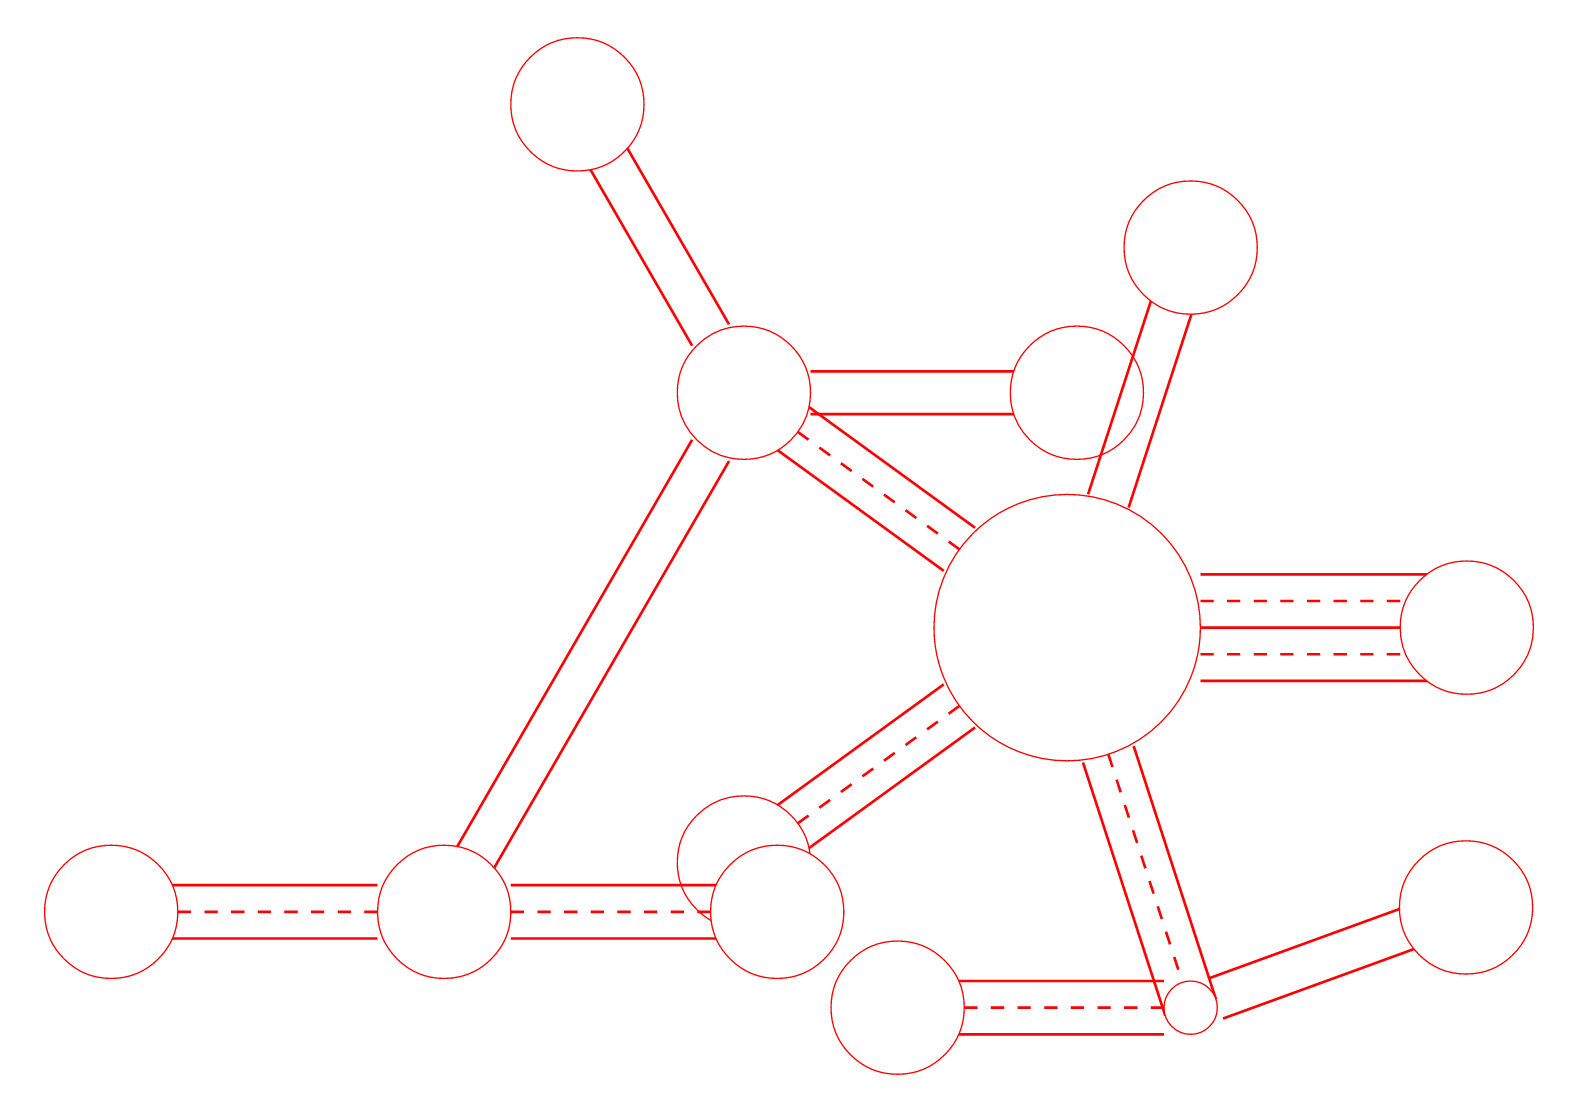
\includegraphics[width=12cm, height=9.5cm]{roadnet.png}

\section{Future Considerations}

The original plan was to draw the intersections such that no overlapping paths would exist. Because of time constraints and technical difficulties involving the storage and retrieval of x and y coordinates pushed onto a stack and then popped, this wasn't done. For the future, a nice feature would be to add Bezier curves to link each road link within an intersection to eachother, as in a real top-down view of a road network. SVG has native support for Bezier curves.

\end{document}
